\section{Conceptual Introduction---Transformers and Attention for Beginners}
\label{sec:annex-tutorial}

This appendix is the on-ramp to the paper: it explains what a transformer is and how attention works, for readers with no deep-learning background. Every mechanism is introduced through one real-world analogy, and --- this is the point of the appendix --- the \emph{same} analogy returns every time the mechanism returns, so a single mental image carries you from the first intuition to the mathematics. Table~\ref{tab:tut-analogies} lists the cast; the running example is always the same sentence, ``The cat eats fish''.

\begin{table}[H]
\centering
\begin{tabular}{@{}lll@{}}
\toprule
\textbf{Mechanism} & \textbf{Analogy reused throughout} & \textbf{Introduced in}\\
\midrule
Attention & listening to one voice in a noisy room & \S\ref{subsec:tut-attention}\\
Queries, keys, values & visitor, catalog card, and book in a library & \S\ref{subsec:tut-math}\\
Attention heads & a team of analysts, one question each & \S\ref{subsec:tut-heads}\\
Stacked layers & editing an essay in successive passes & \S\ref{subsec:tut-layers}\\
\bottomrule
\end{tabular}
\caption{The cast of analogies of this tutorial. Each row is introduced once and then reused verbatim in every later section, including the takeaways.}
\label{tab:tut-analogies}
\end{table}

\subsection{What Is a Transformer? Words in Context}
\label{subsec:tut-context}

A transformer is a neural architecture that processes text (or any sequence) by interpreting the meaning of each word \emph{in the light of all the other words around it}. The problem it solves is easiest to see with an ambiguous word. Read this:

\begin{center}
\textit{``The bank was full of people waiting. Mary went to the bank.''}
\end{center}

What does ``bank'' mean in each case? Taken alone, the word has three unrelated meanings: a financial institution, a bench to sit on, the ground beside a river. Inside the first sentence, the neighbors (``full of people waiting'') vote for the branch office. Inside the second, ``Mary went to the\ldots'' leaves two readings alive --- she could be heading to the counter or to the river. Figure~\ref{fig:tut-context} contrasts the two situations.

\begin{figure}[H]
\centering
\fitfigure{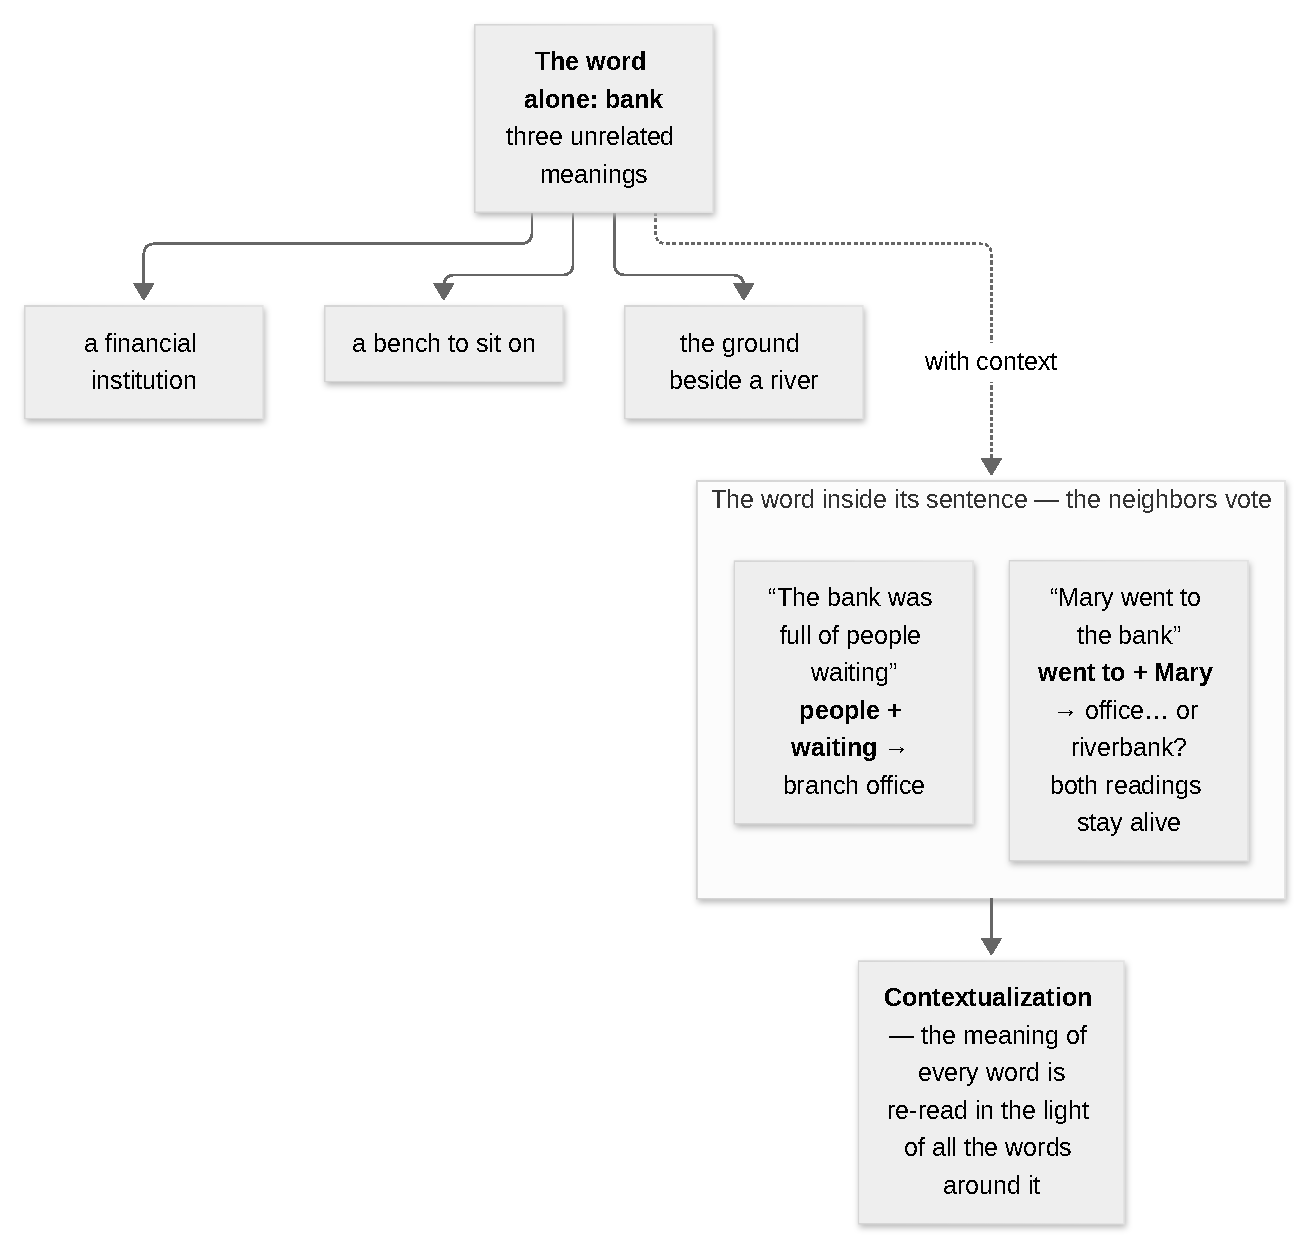
\includegraphics{figures/tutorial/tutorial-context.pdf}}
\caption{Contextualization in one picture: the word ``bank'' alone has three unrelated meanings (top); inside its sentence, the neighboring words vote and select the reading (middle). A transformer does this for every word simultaneously.}
\label{fig:tut-context}
\end{figure}

This ability to re-read every word in the light of the whole sentence is called \emph{contextualization}, and it is the heart of every modern transformer. The question this appendix answers is \emph{how} the model decides which neighbors to listen to. The answer is attention.

\subsection{The Attention Mechanism: One Voice in a Noisy Room}
\label{subsec:tut-attention}

Attention is the ``magic trick'' behind contextualization. Think of a conversation in a noisy room:

\begin{enumerate}[leftmargin=*]
    \item \textbf{Lots of noise}: many people talk at once, but one of them matters to you.
    \item \textbf{You ignore the rest}: your brain automatically focuses on that one voice and filters the rest.
    \item \textbf{You understand better}: by concentrating, you catch every word clearly.
\end{enumerate}

The neural mechanism works the same way, with one twist: \emph{every word in the sentence is such a listener}. Each word ``asks'' how important every other word is for understanding it, then focuses its attention on the most relevant ones. The room is the sentence, the voices are the words, and the focusing ability is attention. Keep this image: every formula below is just the arithmetic version of listening selectively.

\subsection{A Worked Example: The Two Lives of ``eats''}
\label{subsec:tut-example}

Let us watch the mechanism work on one word in two different sentences. The numbers that follow are illustrative, but they are exactly the kind of table a trained transformer computes --- Figure~\ref{fig:tut-heatmap} shows both cases.

\subsubsection{Context 1: ``The cat eats fish''}

Processing ``eats'', the word-as-listener asks about every other voice in the room:
\begin{itemize}[leftmargin=*]
    \item How relevant is ``The''? Little --- it is just an article. \textbf{Low attention: 5\%}.
    \item How relevant is ``cat''? Very --- it is the subject, who eats. \textbf{High attention: 55\%}.
    \item How relevant is ``eats''? A little --- itself. \textbf{Low attention: 5\%}.
    \item How relevant is ``fish''? Very --- it is what gets eaten. \textbf{High attention: 35\%}.
\end{itemize}
The new representation of ``eats'' is dominated by ``cat'' and ``fish'': an action, with its subject and its object.

\subsubsection{Context 2: ``The restaurant eats into profit margins''}

Same word, different room. Now the listeners that matter are different:
\begin{itemize}[leftmargin=*]
    \item ``restaurant'' (the subject): \textbf{30\%}.
    \item ``profit'' (what is affected): \textbf{25\%}.
    \item ``margins'' (what gets consumed): \textbf{35\%}.
    \item ``The'', ``into'', and ``eats'' itself: the remaining \textbf{10\%}.
\end{itemize}

\begin{figure}[H]
\centering
\fitfigure{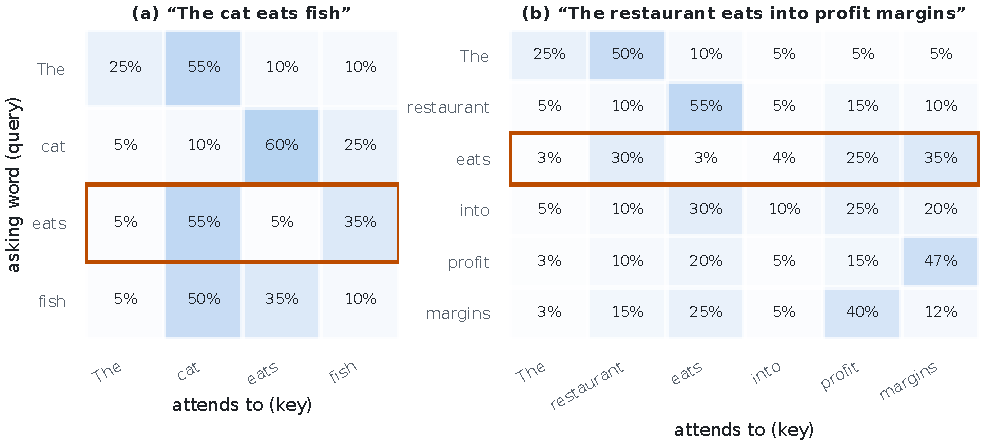
\includegraphics{figures/tutorial/tut-attention-heatmap.pdf}}
\caption{Two attention matrices (rows: asking word; columns: word attended to; the highlighted row is ``eats''). In (a) the word ``eats'' listens mostly to ``cat'' (55\%) and ``fish'' (35\%); in (b) the same word listens to ``restaurant'', ``profit'' and ``margins''. Same word, different room, different focus --- contextualization in action. Every row sums to 100\% because attention is a limited budget.}
\label{fig:tut-heatmap}
\end{figure}

The word ``eats'' ends up with a completely different representation in each sentence because it \emph{attends} to different words. That is the whole trick: one word, many possible meanings, and attention picking the right neighbors to define it.

\subsection{How Attention Works Mathematically: A Library Called Attention}
\label{subsec:tut-math}

Behind the listening there is arithmetic. The standard analogy --- and the one this paper sticks to --- is a library, shown in Figure~\ref{fig:tut-qkv}.

\begin{figure}[H]
\centering
\fitfigure{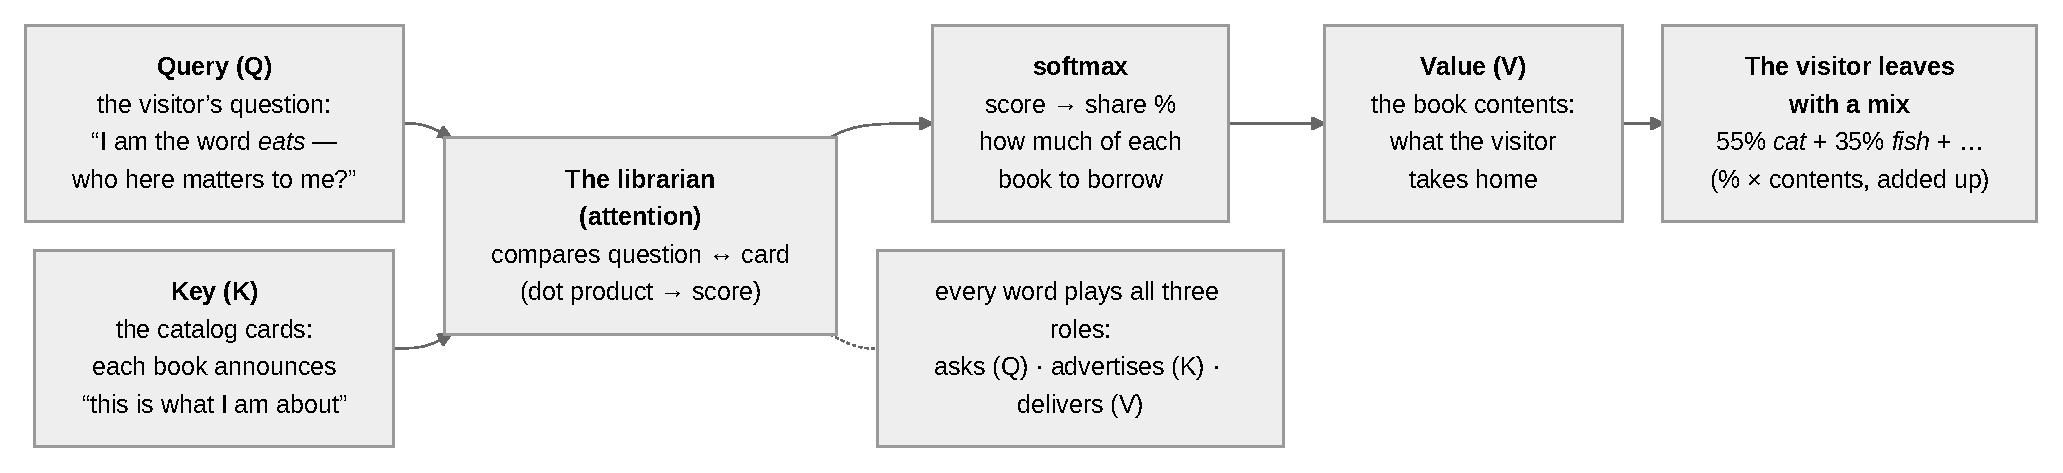
\includegraphics{figures/tutorial/tutorial-qkv-library.pdf}}
\caption{Queries, keys and values as a library visit. The visitor carries a question (Q), every book advertises itself with a catalog card (K), the librarian compares question and cards (the attention), and the visitor leaves with a weighted mix of the book contents (V).}
\label{fig:tut-qkv}
\end{figure}

\subsubsection{Step 1: Queries, Keys, and Values}

Each word is transformed into three versions of itself:
\begin{itemize}[leftmargin=*]
    \item \textbf{Query (Q)}: the visitor's question --- ``what information do I need?''
    \item \textbf{Key (K)}: the catalog card --- ``what information do I offer?''
    \item \textbf{Value (V)}: the book's content --- ``here is my actual information.''
\end{itemize}
Crucially, every word plays all three roles at once: it asks (Q), it advertises (K), it delivers (V). One visit to the library, with every book simultaneously a visitor and a shelf.

\subsubsection{Step 2: Compatibility}

The librarian compares the question with every card. Questions similar to a card get a high compatibility score; the score is computed by multiplying the query by the key (a \emph{dot product}). For our ``eats'' query: $\mathrm{s}(\text{eats} \rightarrow \text{cat}) = 3.40$, $\mathrm{s}(\text{eats} \rightarrow \text{fish}) = 2.95$, $\mathrm{s}(\text{eats} \rightarrow \text{The}) = 1.00$. Figure~\ref{fig:tut-attention-steps} places the four steps in one pipeline.

\begin{figure}[H]
\centering
\fitfigure{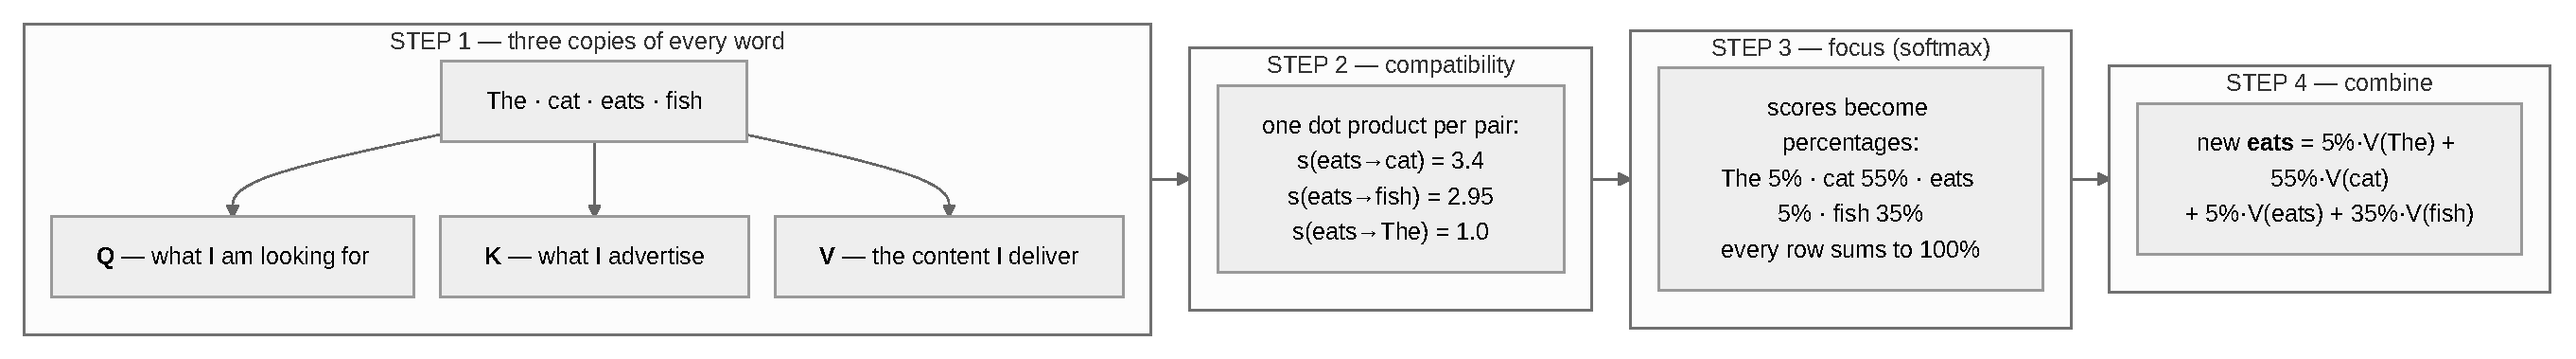
\includegraphics{figures/tutorial/tutorial-attention-steps.pdf}}
\caption{The full attention step for the query ``eats'' in ``The cat eats fish'': three copies per word (Step 1), one dot product per query--key pair (Step 2), softmax turning scores into percentages (Step 3), and the weighted combination of values (Step 4). The numbers are the same as in Figures~\ref{fig:tut-heatmap} and~\ref{fig:tut-softmax}.}
\label{fig:tut-attention-steps}
\end{figure}

\subsubsection{Step 3: Focus}

Raw scores are just numbers; attention is a \emph{budget}. A function called \texttt{softmax} converts the scores into percentages that always sum to 100\%: the ``eats'' query turns the scores above into \textbf{5\% / 55\% / 5\% / 35\%} over ``The / cat / eats / fish''. Figure~\ref{fig:tut-softmax} shows the conversion. High compatibility means ``focus attention here''; low compatibility means ``ignore this'' --- back in the noisy room, the voice you decided to filter out.

\begin{figure}[H]
\centering
\fitfigure{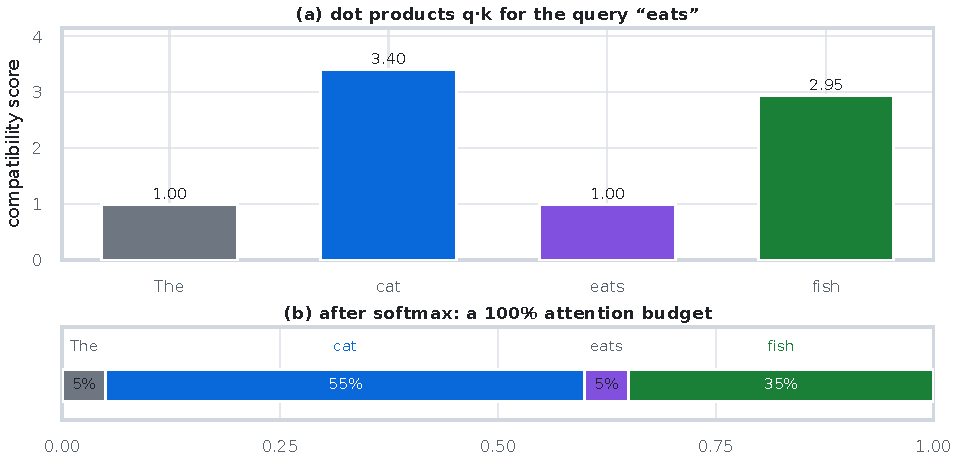
\includegraphics{figures/tutorial/tut-softmax-focus.pdf}}
\caption{Step 2 $\rightarrow$ Step 3 in numbers. Top: the four raw compatibility scores (dot products) for the query ``eats''. Bottom: after \texttt{softmax}, the same four numbers become an attention budget that sums to exactly 100\%.}
\label{fig:tut-softmax}
\end{figure}

\subsubsection{Step 4: Combine}

Finally the visitor leaves the library with a weighted mix of contents. If ``eats'' places 55\% of its budget on ``cat'' and 35\% on ``fish'', then 55\% of cat's value and 35\% of fish's value are blended into the new representation of ``eats'':
\begin{equation}
\text{new ``eats''} \;=\; 5\%\cdot v_{\text{The}} + 55\%\cdot v_{\text{cat}} + 5\%\cdot v_{\text{eats}} + 35\%\cdot v_{\text{fish}}.
\label{eq:tut-mix}
\end{equation}
That blended vector is what the rest of the network sees: a representation of ``eats'' that already contains who eats and what gets eaten.

\subsection{Multiple Attention Heads: A Team of Analysts}
\label{subsec:tut-heads}

Transformers never run one attention but \emph{many heads in parallel} --- as if the sentence were analyzed by a team of specialists, each asking a different question about it (Figure~\ref{fig:tut-heads}):

\begin{itemize}[leftmargin=*]
    \item \textbf{Analyst 1 (grammar)}: ``who does it?'' --- links \emph{cat} $\rightarrow$ \emph{eats}.
    \item \textbf{Analyst 2 (object)}: ``what receives it?'' --- links \emph{eats} $\rightarrow$ \emph{fish}.
    \item \textbf{Analyst 3 (time)}: ``when / how often?'' --- tracks verb tense and time words.
    \item \textbf{Analyst 4 (style)}: ``which articles and modifiers?'' --- tracks ``the'', ``a'', adjectives.
\end{itemize}

\begin{figure}[H]
\centering
\fitfigure{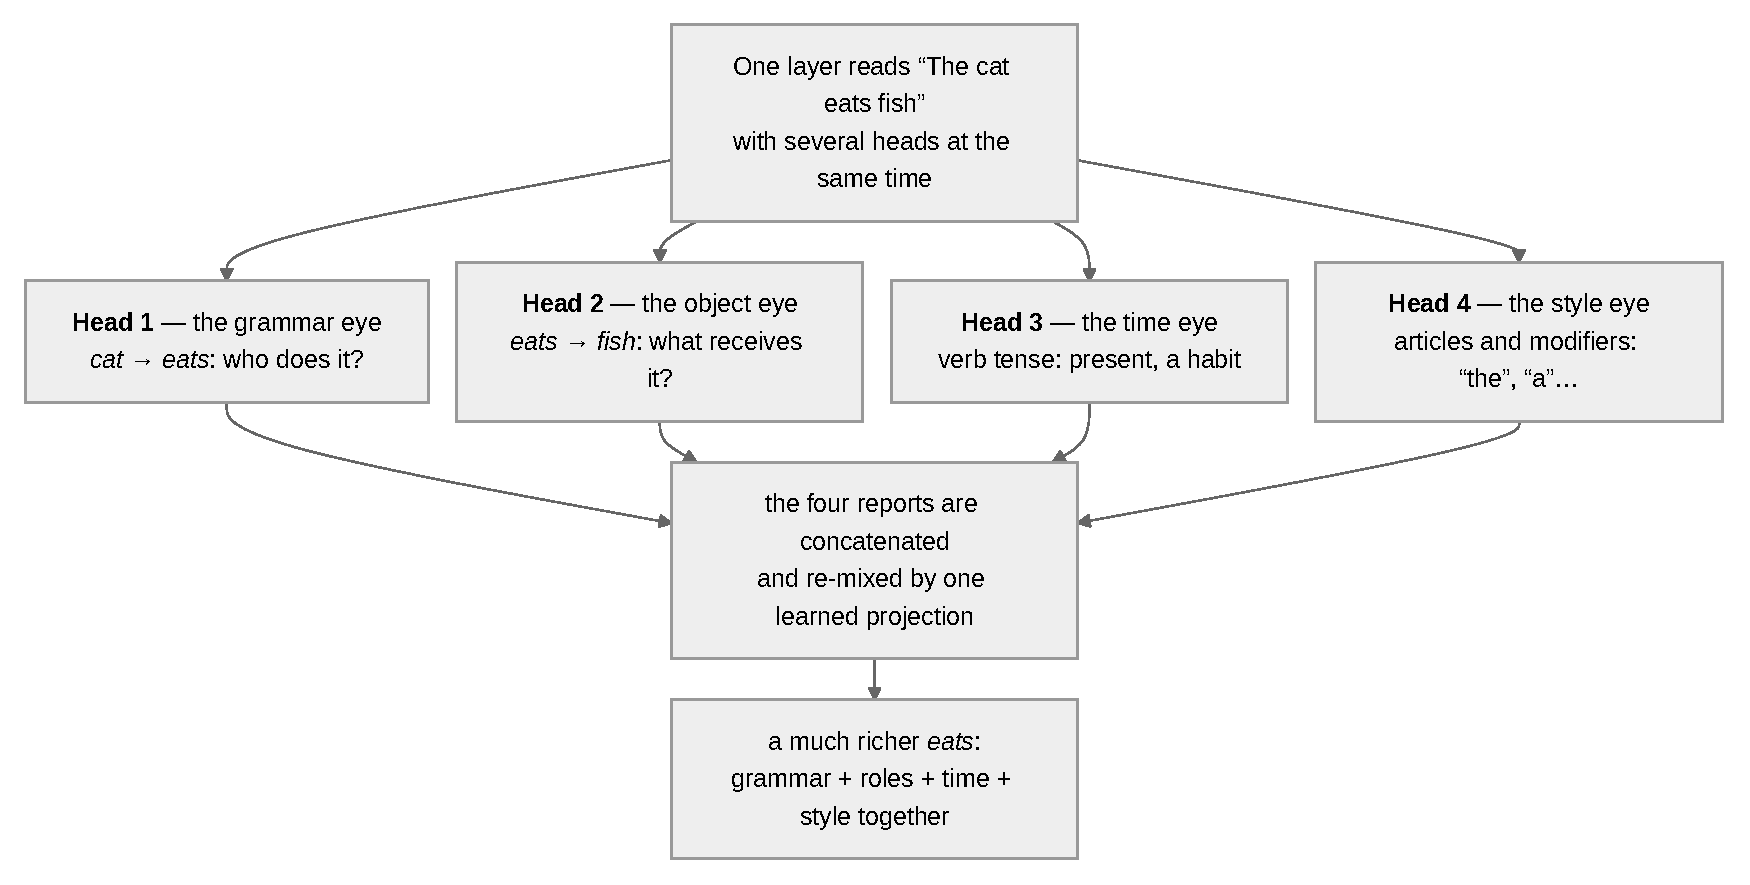
\includegraphics{figures/tutorial/tutorial-heads.pdf}}
\caption{Several heads read the same sentence simultaneously, like a team of analysts with one question each. Their reports are concatenated and re-mixed into a single, much richer representation.}
\label{fig:tut-heads}
\end{figure}

Each head learns its own focus pattern from data, and their reports are concatenated and re-mixed by one learned projection. Together they capture far more than any single head could --- grammar, roles, time and style at once.

\subsection{Stacking Layers: Editing the Essay in Passes}
\label{subsec:tut-layers}

One attention step still sees shallow patterns, so transformers stack the same block many times (12 to 48 in practical models). The analogy: editing an essay in successive passes (Figure~\ref{fig:tut-layers}).

\begin{enumerate}[leftmargin=*]
    \item \textbf{First pass} --- fix spelling and basic grammar: recognize words, forms, gender.
    \item \textbf{Second pass} --- improve clarity of each sentence: who does what to whom.
    \item \textbf{Third pass} --- ensure consistency and narrative flow: idioms, relations, abstract meaning.
\end{enumerate}

\begin{figure}[H]
\centering
\fitfigure{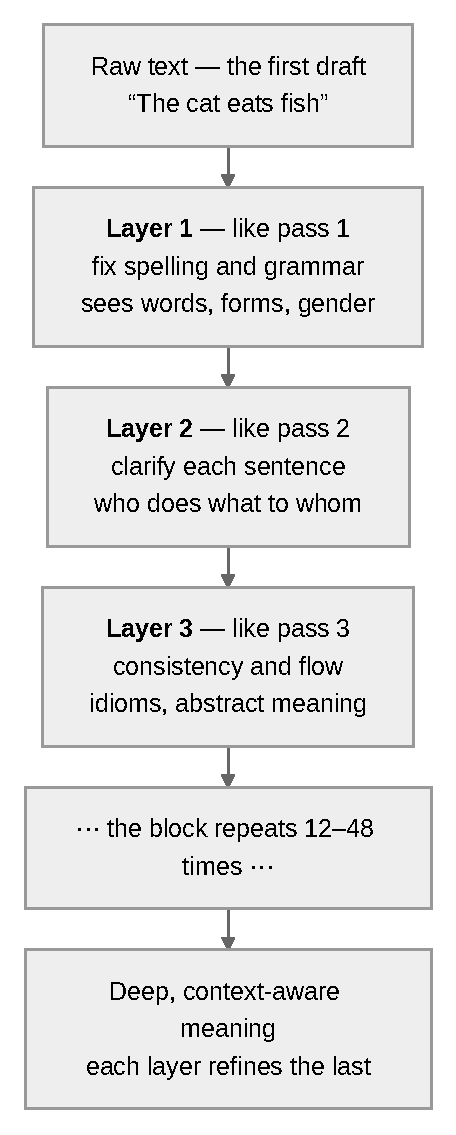
\includegraphics{figures/tutorial/tutorial-layers.pdf}}
\caption{Layers as editing passes: the raw text enters at the top and each layer refines the previous layer's reading --- from words and forms, through sentence structure, to abstract meaning. The block repeats 12--48 times in practice.}
\label{fig:tut-layers}
\end{figure}

Each layer re-reads what the previous layer produced and refines it: early layers capture basic features, later layers understand complex relations and abstract concepts. No layer is told what to look for --- the passes organize themselves during training.

\subsection{Why Does It Matter?}

The attention mechanism was revolutionary because:
\begin{enumerate}[leftmargin=*]
    \item \textbf{Parallelism}: any word can be compared with any other word \emph{at once} (no sequential processing, unlike earlier recurrent systems) --- fast on modern hardware.
    \item \textbf{Flexibility}: the patterns are learned from data; nobody programs the rules.
    \item \textbf{Scalability}: the same mechanism works from a sentence to millions of words of context.
    \item \textbf{Generality}: translation, summarization, question answering, generation, computer vision, audio --- one mechanism, many tasks.
\end{enumerate}

\subsection{Practical Challenges: The Price of Listening to Everyone}
\label{subsec:tut-challenges}

Dense attention buys its power by comparing \emph{every} word with \emph{every} other word, and that price grows fast.

\subsubsection{Computational Complexity}

A 1,000-word document forces $1{,}000 \times 1{,}000 = 1{,}000{,}000$ word-to-word comparisons, and the cost squares as the document grows. Figure~\ref{fig:tut-complexity} shows the growth against the friendlier alternatives discussed below.

\begin{figure}[H]
\centering
\fitfigure{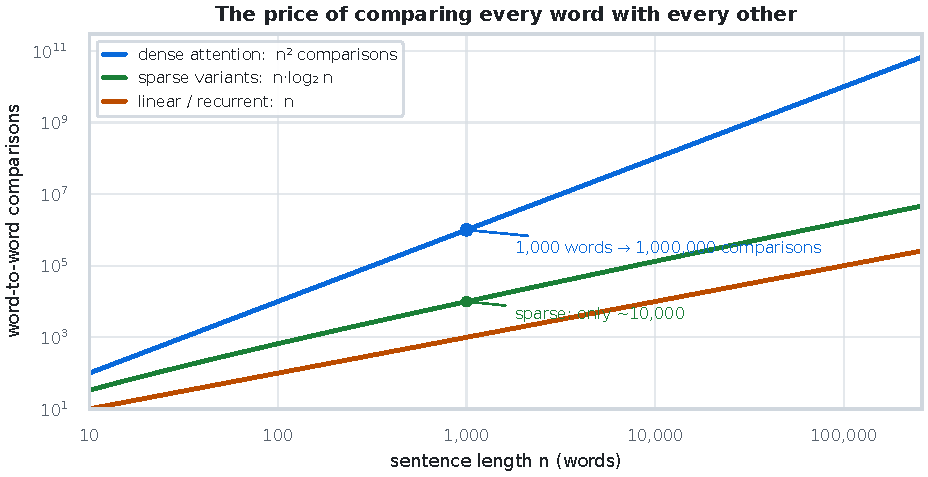
\includegraphics{figures/tutorial/tut-complexity-growth.pdf}}
\caption{Word-to-word comparisons versus sentence length. Dense attention compares every word with every other ($n^2$): at $n = 1{,}000$ that is already one million comparisons. Sparse variants ($n \log_2 n$) and linear-time / recurrent models ($n$) grow far more gently.}
\label{fig:tut-complexity}
\end{figure}

\subsubsection{Memory Requirements}

During inference (using a trained model), the keys and values of every past word must be stored --- the library keeps every book on the table just in case a later query needs it. For long contexts this cache dominates GPU memory.

\subsubsection{Device Efficiency}

Transformers were designed for powerful TPUs and GPUs; running them on phones or embedded devices is challenging.

\subsection{Modern Solutions: Smarter Ways to Listen}
\label{subsec:tut-solutions}

The rest of this paper is a catalog of ways to keep the benefits of attention while paying less. Each keeps our analogies:

\begin{itemize}[leftmargin=*]
    \item \textbf{Sparse attention}: stop browsing \emph{every} card in the library --- visit only nearby shelves and a few strategic ones. Complexity drops from $\mathcal{O}(n^2)$ to $\mathcal{O}(n \log n)$ or $\mathcal{O}(n)$.
    \item \textbf{Recurrent models} (e.g.\ Mamba): take notes as you read, instead of re-listening to the whole room for every new word --- an old idea (recurrence) rebuilt with modern efficiency.
    \item \textbf{Gated attention}: a gatekeeper decides which of your notes are worth keeping and which to fade out, so less needs to be stored.
    \item \textbf{Quantization}: write each number with fewer digits (small integers instead of wide decimals), shrinking memory with minimal loss of precision.
\end{itemize}

These innovations are exactly what this toolkit (Frankenstein) lets you experiment with, and the annexes that follow are guided tours of each family.

\subsection{Key Takeaways}

\begin{itemize}[leftmargin=*]
    \item A \textbf{transformer} is a network that contextualizes: it re-reads every word in the light of all its neighbors (the ambiguous ``bank'').
    \item \textbf{Attention} is selective listening: each word focuses its limited 100\% budget on the neighbors that define it (the noisy room).
    \item The arithmetic is a library visit: \textbf{query} asks, \textbf{key} advertises, \textbf{value} delivers; dot products score compatibility, \texttt{softmax} turns scores into a 100\% budget, and the values are mixed by that budget.
    \item \textbf{Multiple heads} are a team of analysts with one question each; \textbf{stacked layers} are successive editing passes, each refining the last.
    \item The catch: dense attention compares everyone with everyone --- $\mathcal{O}(n^2)$ --- which is why sparse, recurrent, gated and quantized variants exist.
    \item Every later annex of this paper is a deeper tour of one of those variants; the analogies of Table~\ref{tab:tut-analogies} will keep coming back.
\end{itemize}
